
\documentclass[11pt,a4paper]{article}

% ==============================
% 📦 PACKAGES
% ==============================

\usepackage[utf8]{inputenc}
\usepackage[T1]{fontenc}
\usepackage{lmodern}
\usepackage{geometry}
\usepackage{amsmath, amssymb, amsthm}
\usepackage{mathtools}
\usepackage{graphicx}
\usepackage{float}
\usepackage{booktabs}
\usepackage{array}
\usepackage{enumitem}
\usepackage{xcolor}
\usepackage{hyperref}
\usepackage{tikz}
\usepackage{pgfplots}
\usepackage{listings}
\usepackage{tcolorbox}
\usepackage{tikz}
\usepackage[american]{circuitikz}
\pgfplotsset{compat=1.18}

% ==============================
% 📐 PAGE STYLE
% ==============================

\geometry{
    left=2.5cm,
    right=2.5cm,
    top=2.5cm,
    bottom=2.5cm
}

\setlength{\parindent}{0pt}
\setlength{\parskip}{6pt}

% ==============================
% 🎨 COLOR PALETTE (Minimal & Elegant)
% ==============================

\definecolor{mainblue}{RGB}{25,55,109}
\definecolor{lightgray}{RGB}{245,245,245}

% ==============================
% 📦 THEOREM ENVIRONMENTS
% ==============================

\newtheorem{theorem}{Teorema}[section]
\newtheorem{definition}{Definizione}[section]
\newtheorem{proposition}{Proposizione}[section]
\newtheorem{example}{Esempio}[section]

% ==============================
% 🧠 CUSTOM BOXES (Very Clean)
% ==============================

\newtcolorbox{importantbox}{
    colback=lightgray,
    colframe=mainblue,
    boxrule=0.8pt,
    arc=4pt
}

% ==============================
% 💻 CODE STYLE
% ==============================

\lstset{
    language=C++, % cambia se vuoi (Python, Java, ecc.)
    basicstyle=\ttfamily\small,
    keywordstyle=\color{blue},
    commentstyle=\color{gray},
    stringstyle=\color{red},
    numbers=left,
    numberstyle=\tiny,
    stepnumber=1,
    numbersep=8pt,
    backgroundcolor=\color{lightgray},
    frame=single,
    breaklines=true
}

% ==============================
% 📄 DOCUMENT
% ==============================

\begin{document}
% ==============================
\section{lezione del 24-03-26}
\subsection{Il transistore bipolare BJT}\label{sub:il_transistore_bipolare_bjt} % (fold)
Il \textit{Bipola Junction Transistore}(\textbf{BJT}) è un dispositovo \textbf{attivo} a due porte e tre terminali.
Viene idealmente rappresentato come un generatore di corrente controllato in corrente (\textbf{Modello GCCC}).
Nel suo uso generico si accoppia una rete esterna che comprende un generatore di segnale di bassa potenza e di carico.
\begin{center}
    \begin{circuitikz}
        \draw (0,0) to[voltage source, l=$v_S$, invert] (0, 2)
        (0,2) to[resistor, l=$R_S$, i>=$i_1$] (4,2)
        (0,0) -- (6,0)
        (4,0) to[short, v^<=$v_1$] (4,2)
        (6,0) to[american controlled current source,l_=$A_i i_1$, invert](6, 2)
        (6,2) to[short, i<=$i_2$](10,2)
        (6,0) -- (10,0)
        (10,0) to[resistor, l_=$R_L$, v^<=$v_2$] (10,2);
    \end{circuitikz} 
\end{center}
Questo circuito è  costituito da una \textit{rete sorgente}(parte sinistra) e una \textit{rete di carico} (parte destra). 
A sinistra del circuito troviamo:
\begin{itemize}
    \item Generatore di tensione sorgente $v_S$
    \item Resistenza sorgente $R_S$

\end{itemize}
Il generatore impone una tensione ai capi della resistenza, questo porta a far si che sulla resistenza ci scorra una corrente 
che chiameremo $i_1$. 

A destra troviamo:
\begin{itemize}
    \item Generatore di corrente controllato in corrente $A_i i_1$ 
    \item Resistenza di carico $R_L$
\end{itemize}
Un transitore bipolare sarà quindi un circutio che accetta una corrente a sinistra e impone una corrente modulata a destra.
% subsection Il transistore bipolare BJT (end)

\subsubsection{Guadagno di tensione e corrente}\label{sec:guadagno_di_tensione_e_corrente} % (fold)
Vediamo nel dettaglio cosa rappresenza il parametro $A_i$.
\begin{itemize}
    \item \textbf{Guadagno in corrente $A_i$}: guardando alla maglia a destra notiamo che
        \[
            i_2 = A_i i_1 \implies A_i = \frac{i_2}{i_1}
        \]
    \item \textbf{Guadagno in tensione $A_v$}: il collegamento alla rete esterna (indicata dalla
        resistenza $R_L$) ci permette di definite questo guadagno come
        \[
            v_2 = -R_L i_2 = -R_L A_i i_1 
        \]
        Applicando la seconda legge di Kirchhoff alla maglia sinistra otteniamo
        \[
            i_1 = \frac{v_S}{R_S}
        \]
        Sostituendo il valore di $i_1$ trovato nell'equazione precendente 
        \[
            v_2 = -R_L A_i \frac{v_s}{R_S}
        \]

        Quello che vogliamo è esplicitare il guadagno di tensione definito come rapporto
        fra la differenza di potenziale sulla \textit{reisistenza di carico} e la tensione del \textit{generatore sorgente}
        \[
            A_v = \frac{v_2}{v_S} = -A_i\frac{R_L}{R_S}
        \]
\end{itemize}
Questi guadagni vengono detti di \textit{amplificazione} o di \textit{attenuazione} in base ai loro valori
$$
    A_i = \frac{i_\mathrm{out}}{i_\mathrm{in}} \quad \text{(guadagno di corrente)} \quad
    \begin{cases}
        A_i > 1 \quad \text{(amplificazione di corrente)} \\
        A_i < 1 \quad \text{(attenuazione di corrente)}
    \end{cases}
    $$
    \[
    A_v = \frac{v_\mathrm{out}}{v_\mathrm{in}} \quad \text{(guadagno di tensione)} \quad
    \begin{cases}
        A_v > 1 \quad \text{(amplificazione di tensione)} \\
        A_v < 1 \quad \text{(attenuazione di tensione)}
    \end{cases}
    \]
\subsubsection{Guadagno di potenza}\label{sec:guadagno_di_potenza} % (fold)
Facciamo delle considerazione anche sulla potenza erogata dal circuito. 
\begin{itemize}
    \item Sul \textit{carico} viene erogata una potenza pari a 
        \[
            P_L = -v_2 i_2
        \]
    \item La \textit{sorgente} eroga una potenza pari a 
        \[
            P_S = v_S i_1
        \]
\end{itemize}
Possiamo quindi definire un guadagno di potenza 
\[
    A_P = \frac{P_L}{P_S} = - \frac{v_2 i_2}{v_S i_1} = -A_i A_v = A_i^2\frac{R_L}{R_S}
\]

Notiamo quindi una prima particolarità dei transistor: i componenti \textit{attivi} (come i \textbf{BJT} o i \textbf{MOSFET}, \textit{Metal–Oxide–Semiconductor Field-Effect Transistor}) permettono di ottenere valori di $A_P > 1$, cioè ricavare più potenza al carico di quanta ne viene erogata dalla sorgente (chiaramente sotto alimentazione esterna).
Questo è il primo caso di utilizzo del transistor, cioè come \textit{amplificatore} di potenza.
% subsubsection Guadagno di potenza (end)
\subsection{Trattazione fisica del transitore bipolare}\label{sub:trattazione_fisica_del_transitore_bipolare} % (fold)
Abbiamo visto elettronicamente come è composto e quali sono i principali scopi di un transitore bipolare
analizzando i guadagni di \textit{tensione}, \textit{corrente} e \textit{potenza}. 
Concentriamoci adesso sulla realizzazione fisica di questo componente.

Il transitore bipolare a giunzione consiste di due giunzioni \textbf{p-n} poste l'una di fianco
all'altra orientate in senso inverso. Si possono quindi ottenere due diverse configurazioni 
\textbf{pnp} oppure \textbf{npn}.
\begin{center}
    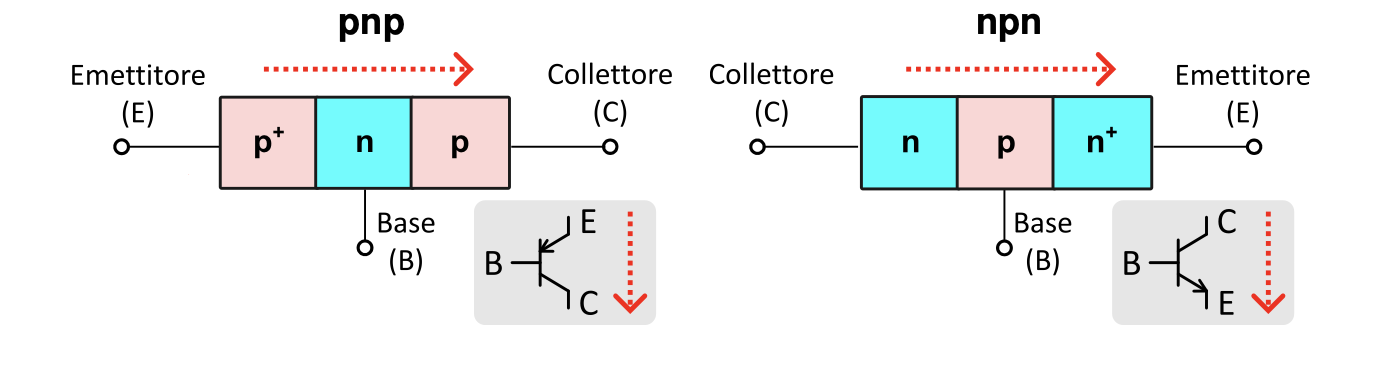
\includegraphics[scale=0.45]{../images/transitore_bipolare.png} 
\end{center}
Notiamo la presenza di tre componenti: 
\begin{itemize}
    \item \textbf{Emettitore}: emette i portatori di carica
    \item \textbf{Collettore}: raccoglie i portatori di carica
    \item \textbf{Base}: modula/controlla il passaggio dei portatori
\end{itemize}
Il drogaggio delle varie sezioni non è uguale, le sezioni che hanno un segno $+$ come apice 
sono significativamente più drogate delle loro corrispettive. Questo come andremo a vedere permette
il coretto funzionamento da transitore del componente.
I versi indicati delle correnti in entrambe le configurazioni sono i versi \textit{naturali}
durante il funzionamento da \textit{GCCC}.
% subsection Trattazione fisica del transitore bipolare (end)
\end{document}

